\section{Tutorial A12}

\begin{problem}
    $A$ and $B$ are two independent events such that $\P{A} = 0.2$ and $\P{B} = 0.15$. Evaluate the following probabilities.
    \begin{enumerate}
        \item $\P{A}{B}$,
        \item $\P{A \cap B}$,
        \item $\P{A \cup B}$.
    \end{enumerate}
\end{problem}
\begin{solution}
    \begin{ppart}
        Since $A$ and $B$ are independent, $\P{A}{B} = \P{A} = 0.2$.
    \end{ppart}
    \begin{ppart}
        Since $A$ and $B$ are independent, $\P{A \cap B} = \P{A}\P{B} = 0.2 \cdot 0.15 = 0.03$.
    \end{ppart}
    \begin{ppart}
        $\P{A \cup B} = \P{A} + \P{B} - \P{A \cap B} = 0.2 + 0.15 - 0.03 = 0.32$.
    \end{ppart}
\end{solution}

\begin{problem}
    Two events $A$ and $B$ are such that $\P{A} = \frac{8}{15}$, $\P{B} = \frac{1}{3}$ and $\P{A}{B} = \frac15$. Calculate the probabilities that
    \begin{enumerate}
        \item both events occur,
        \item only one of the two events occurs,
        \item neither event occurs.
    \end{enumerate}
    Determine if event $A$ and $B$ are mutually exclusive or independent.
\end{problem}
\begin{solution}
    \begin{ppart}
        \[\P{A \cap B} = \P{B} \P{A}{B} = \frac13 \cdot \frac15 = \frac1{15}.\]
    \end{ppart}
    \begin{ppart}
        \begin{gather*}
            \P{\text{only one occurs}} = \P{A \cup B} - \P{A \cap B} = \P{A} + \P{B} - 2\P{A \cap B} \\
            = \frac8{15} + \frac13 - 2 \bp{\frac1{15}} = \frac{11}{15}.
        \end{gather*}
    \end{ppart}
    \begin{ppart}
        \[\P{\text{neither occurs}} = 1 - \P{\text{at least one occurs}} = 1 - \bp{\frac1{15} - \frac{11}{15}} = \frac15.\]
    \end{ppart}

    Since $\P{A} = \frac8{15} \neq \frac15 = \P{A}{B}$, it follows that $A$ and $B$ are not independent. Also, since $\P{A \cap B} = \frac1{15} \neq 0$, the two events are also not mutually exclusive.
\end{solution}

\clearpage
\begin{problem}
    Two events $A$ and $B$ are such that $\P{A} = \P{B} = p$ and $\P{A \cup B} = \frac59$.
    \begin{enumerate}
        \item Given that $A$ and $B$ are independent, find a quadratic equation satisfied by $p$.
        \item Hence, find the value of $p$ and the value of $\P{A \cap B}$.
    \end{enumerate}
\end{problem}
\begin{solution}
    \begin{ppart}
        Since $A$ and $B$ are independent, we have $\P{A}{B} = \P{A} = p$. Hence,
        \begin{gather*}
            p = \P{A}{B} = \frac{\P{A \cap B}}{\P{B}} = \frac{\P{A} + \P{B} - \P{A \cup B}}{\P{B}} = \frac{p + p - 5/9}{p} = 2 - \frac{5}{9p}\\
            \implies  9p^2 = 18p - 5 \implies 9p^2 - 18p + 5 = 0.
        \end{gather*}
    \end{ppart}
    \begin{ppart}
        Observe that $9p^2 - 18p + 5 = (3p - 1)(3p - 5)$.  Thus, $p = \frac13$. Note that $p \neq \frac53$ since $0 < p \leq 1$.

        Since $A$ and $B$ are independent, $\P{A \cap B} = \P{A} \P{B} = \frac13 \cdot \frac13 = \frac19$.
    \end{ppart}
\end{solution}

\begin{problem}
    Two players $A$ and $B$ regularly play each other at chess. When $A$ has the first move in a game, the probability of $A$ winning that game is $0.4$ and the probability of $B$ winning that game is $0.2$. When $B$ has the first move in a game, the probability of $B$ winning that game is $0.3$ and the probability of $A$ winning that game is $0.2$. Any game of chess that is not won by either player ends in a draw.
    \begin{enumerate}
        \item Given that $A$ and $B$ toss a fair coin to decide who has the first move in a game, find the probability of the game ending in a draw.
        \item To make their games more enjoyable, $A$ and $B$ agree to change the procedure for deciding who has the first move in a game. As a result of their new procedure, the probability of $A$ having the first move in any game is $p$. Find the value of $p$ which gives $A$ and $B$ equal chances of winning each game.
    \end{enumerate}
\end{problem}
\begin{solution}
    \begin{ppart}
        \begin{align*}
            \P{\text{draw}} &= \P{\text{$A$ first}}\P{\text{draw}}{\text{$A$ first}} + \P{\text{$B$ first}}\P{\text{draw}}{\text{$B$ first}}\\
            &= 0.5 \cdot (1 - 0.4 - 0.2) + 0.5 \cdot (1 - 0.3 - 0.2) = 0.45.
        \end{align*}
    \end{ppart}
    \begin{ppart}
        Observe that 
        \begin{align*}
            \P{\text{$A$ wins}} &= \P{\text{$A$ first}}\P{\text{$A$ wins}}{\text{$A$ first}} + \P{\text{$B$ first}}\P{\text{$A$ wins}}{\text{$B$ first}}\\
            &= p \cdot 0.4 + (1-p) \cdot 0.2 = 0.2p + 0.2
        \end{align*}
        and
        \begin{align*}
            \P{\text{$B$ wins}} &= \P{\text{$A$ first}}\P{\text{$B$ wins}}{\text{$A$ first}} + \P{\text{$B$ first}}\P{\text{$B$ wins}}{\text{$B$ first}}\\
            &= p \cdot 0.2 + (1-p) \cdot 0.3 = -0.1p + 0.3
        \end{align*}
        Consider $\P{\text{$A$ wins}} = \P{\text{$B$ wins}}$. Then $0.2p + 0.2 = -0.1p + 0.3 \implies p = \frac13$.
    \end{ppart}
\end{solution}

\clearpage
\begin{problem}
    Two fair dices are thrown, and events $A$, $B$ and $C$ are defined as follows:
    \begin{itemize}
        \item $A$: the sum of the two scores is odd,
        \item $B$: at least one of the two scores is greater than 4,
        \item $C$: the two scores are equal.
    \end{itemize}
    Find, showing your reasons clearly in each case, which two of these three events are
    \begin{enumerate}
        \item mutually exclusive,
        \item independent.
    \end{enumerate}
    Find also $\P{C}{B}$, making your method clear.
\end{problem}
\begin{solution}
    \begin{ppart}
        Let the scores of the first and second die be $p$ and $q$ respectively. Suppose $A$ occurs. Then $p$ and $q$ are of different parities (e.g. $p$ even $\implies$ $q$ odd). Thus, $p$ and $q$ cannot be equal. Hence, $C$ cannot occur, whence $A$ and $C$ are mutually exclusive.
    \end{ppart}
    \begin{ppart}
        Let the scores of the first and second die be $p$ and $q$ respectively. Observe that $p$ is independent of $q$, and vice versa. Hence, the parity of $q$ is not affected by the parity of $p$. Thus, $\P{A} = \P{\text{$p$ even}}\P{\text{$q$ odd}} + \P{\text{$p$ odd}}\P{\text{$q$ even}} = \frac36 \cdot \frac36 + \frac36 \cdot \frac36 = \frac12$.

        We also have $\P{B} = 1 - \P{\text{neither $p$ nor $q$ is greater than 4}} = 1 - \bp{\frac46}^2 = \frac{20}{36}$.

        \begin{center}
            \begin{tabular}{|c|c|c|c|c|c|c|}
                \hline $p$\textbackslash$q$ & 1 & 2 & 3 & 4 & 5 & 6\\\hline
                1 & 2 & 3 & 4 & 5 & 6 & \cellcolor{blue!25}7 \\ \hline
                2 & 3 & 4 & 5 & 6 & \cellcolor{blue!25}7 & 8 \\ \hline
                3 & 4 & 5 & 6 & 7 & 8 & \cellcolor{blue!25}9 \\ \hline
                4 & 5 & 6 & 7 & 8 & \cellcolor{blue!25}9 & 10 \\ \hline
                5 & 6 & \cellcolor{blue!25}7 & 8 & \cellcolor{blue!25}9 & 10 & \cellcolor{blue!25}11 \\ \hline
                6 & \cellcolor{blue!25}7 & 8 & \cellcolor{blue!25}9 & 10 & \cellcolor{blue!25}11 & 12 \\ \hline
              \end{tabular}
        \end{center}
        
        We now consider $\P(A \cap B)$. From the table of outcomes above, it is clear that $\P(A \cap B) = \frac{10}{36} = \P{A}\P{B}$. Hence, $A$ and $B$ are independent.
    \end{ppart}
\end{solution}

\begin{problem}
    For events $A$ and $B$, it is given that $\P{A} = 0.7$, $\P{B} = 0.6$ and $\P{A}{B'} = 0.8$. Find
    \begin{enumerate}
        \item $\P{A \cap B'}$,
        \item $\P{A \cup B}$,
        \item $\P{B'}{A}$.
    \end{enumerate}
    For a third event $C$, it is given that $\P{C} = 0.5$ and that $A$ and $C$ are independent.
    \begin{enumerate}
        \setcounter{enumi}{3}
        \item Find $\P{A' \cap C}$.
        \item Hence find an inequality satisfied by $\P{A' \cap B \cap C}$ in the form \[p \leq \P{A' \cap B \cap C} \leq q,\] where $p$ and $q$ are constants to be determined.
    \end{enumerate}
\end{problem}
\clearpage
\begin{solution}
    \begin{ppart}
        \[\P{A \cap B'} = \P{B'} \P{A}{B'} = (1-0.6) \cdot 0.8 = 0.32.\]
    \end{ppart}
    \begin{ppart}
        \begin{align*}
            \P{A \cup B} &= \P{A} + \P{B} - \P{A \cap B} = \P{A} + \P{B} - \bs{\P{A} - \P{A \cap B'}}\\
            &= 0.7 + 0.6 - (0.7 - 0.32) = 0.92.
        \end{align*}
    \end{ppart}
    \begin{ppart}
        \[\P{B'}{A} = \frac{\P{B' \cap A}}{\P{A}} = \frac{0.32}{0.7} = \frac{16}{35}.\]
    \end{ppart}
    \begin{ppart}
        Since $A$ and $C$ are independent, $\P{A \cap C} = \P{A} \P{C}$. Hence, $\P{A' \cap C} = \P{C} - \P{A \cap C} = 0.5 - 0.7 \cdot 0.5 = 0.15$.
    \end{ppart}
    \begin{ppart}
        Consider the following Venn diagram.
        \begin{center}
            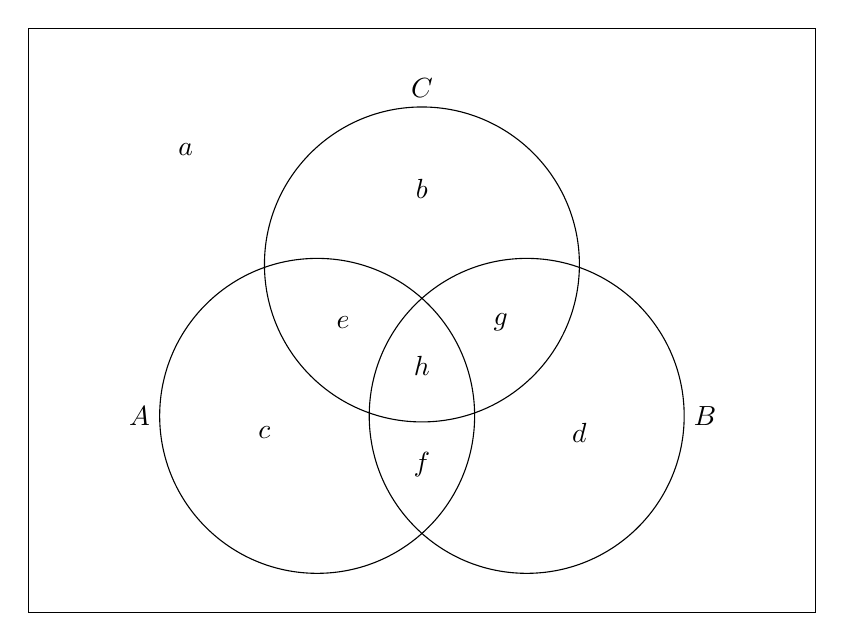
\begin{tikzpicture}
                \coordinate (A) at (-5, -0.5/1.3 - 2.5);
                \coordinate (B) at (5, -0.5/1.3 - 2.5);
                \coordinate (C) at (5, 2/1.3 + 3);
                \coordinate (D) at (-5, 2/1.3 + 3);

                \draw (A) -- (B);
                \draw (B) -- (C);
                \draw (C) -- (D);
                \draw (D) -- (A);

                \draw (0,2/1.3) circle[radius=2];
                \draw (-1.73/1.3,-0.5/1.3) circle[radius=2];
                \draw (1.73/1.3,-0.5/1.3) circle[radius=2];

                \node[left] at (-1.73/1.3 - 2,-0.5/1.3) {$A$};
                \node[right] at (1.73/1.3 + 2,-0.5/1.3) {$B$};
                \node[above] at (0,2/1.3+2) {$C$};

                \node at (-3, 3) {$a$};
                \node at (0, 2.5) {$b$};
                \node at (-2, -0.6) {$c$};
                \node at (2, -0.6) {$d$};
                \node at (-1, 0.8) {$e$};
                \node at (0, -1) {$f$};
                \node at (1, 0.8) {$g$};
                \node at (0, 0.25) {$h$};
            \end{tikzpicture}
        \end{center}

        Note that $\P{A' \cap B \cap C} = g$. Firstly, from part (d), we have $b + g = \P{A' \cap C} = 0.15$. Hence, $g \leq 0.15$. Secondly, from part (b), we have $a + b = 1 - \P{A \cup B} = 1 - 0.92 = 0.08$. Hence, $b \leq 0.08 \implies g \geq 0.07$. Lastly, we know that $\P{A' \cap B} = \P{A \cup B} - \P{A} = 0.92 - 0.7 = 0.22$. Hence, $d + g = 0.22 \implies g \leq 0.22$.

        Thus, $0.07 \leq g \leq 0.15$, whence $0.07 \leq \P{A' \cap B \cap C} \leq 0.15$.
    \end{ppart}
\end{solution}

\begin{problem}
    Camera lenses are made by two companies, $A$ and $B$. 60\% of all lenses are made by $A$ and the remaining 40\% by $B$. 5\% of the lenses made by $A$ are faulty. 7\% of the lenses made by B are faulty.
    \begin{enumerate}
        \item One lens is selected at random. Find the probability that
        \begin{enumerate}
            \item it is faulty,
            \item it was made by $A$, given that it is faulty.
        \end{enumerate}
        \item Two lenses are selected at random. Find the probability that both were made by $A$, given that exactly one is faulty.
        \item Ten lenses are selected at random. Find the probability that exactly two of them are faulty.
    \end{enumerate}
\end{problem}
\begin{solution}
    \begin{ppart}
        \begin{psubpart}
            \[\P{\text{faulty}} = \P{A \cup \text{faulty}} + \P{B \cup \text{faulty}} = 0.6 \cdot 0.05 + 0.4 \cdot 0.07 = 0.058.\]
        \end{psubpart}
        \begin{psubpart}
            \[\P{A}{\text{faulty}} = \frac{\P{A \cap \text{faulty}}}{\P{\text{faulty}}} = \frac{0.6 \cdot 0.05}{0.058} = \frac{15}{19}.\]
        \end{psubpart}
    \end{ppart}
    \begin{ppart}
        \[\P{\text{both $A$}}{\text{one faulty}} = \frac{\P{\text{both $A$} \cup \text{one faulty}}}{\P{\text{one faulty}}} = \frac{\bs{0.6 \cdot 0.05} \cdot \bs{0.6 \cdot (1 - 0.05)}}{0.058 \cdot (1 - 0.058)} = \frac{1425}{4553}.\]
    \end{ppart}
    \begin{ppart}
        \[\P{\text{two faulty}} = 0.058^2 (1 - 0.058)^8 \cdot \frac{10!}{2! 8!} = 0.0939 \tosf{3}\]
    \end{ppart}
\end{solution}

\begin{problem}
    A certain disease is present in 1 in 200 of the population. In a mass screening programme a quick test fo the disease is used, but the test is not totally reliable. For someone who does have the disease there is a probability of $0.9$ that the test will prove positive, whereas for someone who does not have the disease there is a probability of $0.02$ that the test will prove positive.
    \begin{center}
        \begin{tikzpicture}
            \coordinate (A) at (0, 0);
            \coordinate[label=above:diseased] (B1) at (2, 1.5);
            \coordinate[label=below:not diseased] (B2) at (2, -1.5);
            \coordinate[label=right:test positive] (C1) at (5, 2);
            \coordinate[label=right:test negative] (C2) at (5, 1);
            \coordinate (C3) at (5, -1);
            \coordinate (C4) at (5, -2);

            \draw (A) -- (B1);
            \draw (A) -- (B2);
            \draw (B1) -- (C1);
            \draw (B1) -- (C2);
            \draw (B2) -- (C3);
            \draw (B2) -- (C4);

            \node[above left] at ($(A)! 0.5 !(B1)$) {$\frac1{200}$};
        \end{tikzpicture}
    \end{center}
    \begin{enumerate}
        \item One person is selected at random and test.
        \begin{enumerate}
            \item Copy and complete the tree diagram, which illustrates one application of the test.
            \item Find the probability that the person has the disease and the test is positive.
            \item Find the probability that the test is negative.
            \item Given that the test is positive, find the probability that the person has the disease.
        \end{enumerate}
        \item People for whom the test proves positive are recalled and re-tested. Find the probability that a person has the disease if the second test also proves positive.
    \end{enumerate}
\end{problem}
\clearpage
\begin{solution}
    \begin{ppart}
        \begin{psubpart}
            \begin{center}
                \begin{tikzpicture}
                    \coordinate (A) at (0, 0);
                    \coordinate[label=above:diseased] (B1) at (2, 1.5);
                    \coordinate[label=below:not diseased] (B2) at (2, -1.5);
                    \coordinate[label=right:test positive] (C1) at (5, 2);
                    \coordinate[label=right:test negative] (C2) at (5, 1);
                    \coordinate[label=right:test positive] (C3) at (5, -1);
                    \coordinate[label=right:test negative] (C4) at (5, -2);
    
                    \draw (A) -- (B1);
                    \draw (A) -- (B2);
                    \draw (B1) -- (C1);
                    \draw (B1) -- (C2);
                    \draw (B2) -- (C3);
                    \draw (B2) -- (C4);
    
                    \node[above left] at ($(A)! 0.5 !(B1)$) {$\frac1{200}$};
                    \node[below left] at ($(A)! 0.5 !(B2)$) {$\frac{199}{200}$};
                    \node[above] at ($(B1)! 0.6 !(C1)$) {$0.9$};
                    \node[below] at ($(B1)! 0.6 !(C2)$) {$0.1$};
                    \node[above] at ($(B2)! 0.6 !(C3)$) {$0.02$};
                    \node[below] at ($(B2)! 0.6 !(C4)$) {$0.98$};
                \end{tikzpicture}
            \end{center}
        \end{psubpart}
        \begin{psubpart}
            \[\P{\text{diseased} \cap \text{positive}} = \frac1{200} \cdot 0.9 = 0.0045.\]
        \end{psubpart}
        \begin{psubpart}
            \[\P{\text{negative}} = \frac{1}{200} \cdot 0.1 + \frac{199}{200} \cdot 0.98 = 0.9756.\]
        \end{psubpart}
        \begin{psubpart}
            \[\P{\text{diseased}}{\text{positive}} = \frac{\P{\text{diseased} \cap \text{positive}}}{\P{\text{positive}}} = \frac{0.0045}{1 - 0.9756} = 0.184.\]
        \end{psubpart}
    \end{ppart}
    \begin{ppart}
        \begin{align*}
            \text{Required probability} &= \frac{\P{\text{diseased} \cap \text{both positive}}}{\P{\text{both positive}}}\\
            &= \frac{\P{\text{diseased} \cap \text{both positive}}}{\P{\text{diseased} \cap \text{both positive}} + \P{\text{not diseased} \cap \text{both positive}}}\\
            &= \frac{1/200 \cdot 0.9^2}{1/200 \cdot 0.9^2 + 199/200 \cdot 0.02^2} = \frac{2025}{2224}.
        \end{align*}
    \end{ppart}
\end{solution}

\begin{problem}
    In a probability experiment, three containers have the following contents.
    \begin{itemize}
        \item A jar contains 2 white dice and 3 black dice.
        \item A white box contains 5 red balls and 3 green balls.
        \item A black box contains 4 red balls and 3 green balls.
    \end{itemize}
    One die is taken at random from the jar. If the die is white, two balls are taken from the white box, at random and without replacement. If the die is black, two balls are taken from the black box, at random and without replacement. Events $W$ and $M$ are defined as follows:
    \begin{itemize}
        \item $W$: A white die is taken from the jar.
        \item $M$: One red ball and one green ball are obtained.
    \end{itemize}
    Show that $\P{M}{W} = \frac{15}{28}$.

    Find, giving each of your answers as an exact fraction in its lowest terms,
    \begin{enumerate}
        \item $\P{M \cap W}$,
        \item $\P{W}{M}$,
        \item $\P{W \cup M}$.
    \end{enumerate}

    All the dice and balls are now placed in a single container, and four objects are taken at random, each object being replaced before the next one is taken. Find the probability that one object of each colour is obtained.
\end{problem}
\begin{solution}
    Since $W$ has occurred, both red and green balls must come from the white box. Note that there are two ways for $M$ to occur: first a red then a green, or first a green then a red. Hence, $\P{M}{W} = \frac58 \cdot \frac37 + \frac38 \cdot \frac57 = \frac{15}{28}$ as desired.

    \begin{ppart}
        \[\P{M \cup W} = \P{W} \P{M}{W} = \frac25 \cdot \frac{15}{28} = \frac{3}{14}.\]
    \end{ppart}
    \begin{ppart}
        Let $B$ represent the event that a black die is taken from the jar. Then 
        \begin{gather*}
            \P{M} = \P{M \cap W} + \P{M \cap B} = \P{M \cap W} + \P{B} \P{M}{B} \\
            = \frac{3}{14} + \frac35 \bp{\frac47\cdot\frac36 + \frac37\cdot\frac46} = \frac{39}{70}.
        \end{gather*}
        Hence, $\P{W}{M} = \frac{\P{W \cap M}}{\P{M}} = \frac{3/14}{39/70} = \frac5{13}$.
    \end{ppart}
    \begin{ppart}
        \[\P{W \cup M} = \P{W} + \P{M} - \P{W \cap M} = \frac25 + \frac{39}{70} - \frac{3}{14} = \frac{26}{35}.\]
    \end{ppart}

    Note that the container has 2 white objects, 3 black objects, 9 red objects and 6 green objects, for a total of 20 objects. The probability that one object of each colour is taken is thus given by \[\frac2{20} \cdot \frac{3}{20} \cdot \frac9{20} \cdot \frac6{20} \cdot 4! = \frac{243}{5000}.\]
\end{solution}

\begin{problem}
    A man writes 5 letters, one each to $A$, $B$, $C$, $D$ and $E$. Each letter is placed in a separate envelope and sealed. He then addresses the envelopes, at random, one each to $A$, $B$, $C$, $D$ and $E$.
    \begin{enumerate}
        \item Find the probability that the letter to $A$ is in the correct envelope and the letter to $B$ is in an incorrect envelope.
        \item Find the probability that the letter to $A$ is in the correct envelope, given that the letter to $B$ is in an incorrect envelope.
        \item Find the probability that both the letters to $A$ and $B$ are in incorrect envelopes.
    \end{enumerate}
\end{problem}
\clearpage
\begin{solution}
    \begin{ppart}
        \[\P{\text{$A$ correct $\cap$ $B$ incorrect}} = \frac15 \times \frac34 = \frac3{20}.\]
    \end{ppart}
    \begin{ppart}
        \[\P{\text{$A$ correct}}{\text{$B$ incorrect}} = \frac{\P{\text{$A$ correct $\cap$ $B$ incorrect}}}{\P{\text{$B$ incorrect}}} = \frac{3/20}{4/5} = \frac{3}{16}.\]
    \end{ppart}
    \begin{ppart}
        \begin{align*}
            \P{\text{$A$ incorrect $\cap$ $B$ incorrect}} &= \P{\text{$B$ incorrect}} \P{\text{$A$ incorrect}}{\text{$B$ incorrect}}\\
            &= \frac45 \bp{1 - \frac3{16}} = \frac{13}{20}.
        \end{align*}
    \end{ppart}
\end{solution}

\begin{problem}
    A bag contains 4 red counters and 6 green counters. Four counters are drawn at random from the bag, without replacement. Calculate the probability that
    \begin{enumerate}
        \item all the counters drawn are green,
        \item at least one counter of each colour is drawn,
        \item at least two green counters are drawn,
        \item at least two green counters are drawn, given that at least one counter of each colour is drawn.
    \end{enumerate}
    State with a reason whether the events ``at least two green counters are drawn'' and ``at least one counter of each colour is drawn'' are independent.
\end{problem}
\begin{solution}
    \begin{ppart}
        \[\P{\text{all green}} = \frac{\comb64}{10!/(4! \, 6!)} = \frac1{14}.\]
    \end{ppart}
    \begin{ppart}
        \[ \P{\text{one of each colour}} = 1 - \P{\text{all green}} - \P{\text{all red}} = 1 - \frac1{14} - \frac{\comb44}{10!/(4! \, 6!)} = \frac{97}{105}.\]
    \end{ppart}
    \begin{ppart}
        \[\P{\text{at least 2 green}} = 1 - \P{\text{no green}} - \P{\text{one green}} = 1 - \frac1{210} - \frac{\comb61 \cdot \comb43}{10!/(4! \, 6!)} = \frac{37}{42}.\]
    \end{ppart}
    \begin{ppart}
        \[\P{\text{at least 2 green}}{\text{one of each colour}} = \frac{\comb63 \cdot \comb41 + \comb62 \cdot \comb42}{10!/(4! \, 6!) - \comb64 - \comb44}= \frac{85}{97}.\]
    \end{ppart}

    Since $\P{\text{at least 2 green}} = \frac{37}{42} \neq \frac{85}{97} = \P{\text{at least 2 green}}{\text{one of each colour}}$, the two events are not independent.
\end{solution}

\clearpage
\begin{problem}
    A group of fifteen people consists of one pair of sisters, one set of three brothers and ten other people. The fifteen people are arranged randomly in a line.
    \begin{enumerate}
        \item Find the probability that the sisters are next to each other.
        \item Find the probability that the brother are not all next to one another.
        \item Find the probability that either the sisters are next to each other or the brothers are all next to one another or both.
        \item Find the probability that the sisters are next to each other given that the brothers are not all next to one another.
    \end{enumerate}
\end{problem}
\begin{solution}
    \begin{ppart}
        Let the two sisters be one unit. There are hence 14 units altogether, giving $14! \cdot 2!$ arrangements with the restriction. Since there are a total of $15!$ arrangements without the restriction, the required probability is $\frac{14! \cdot 2!}{15!} = \frac{2}{15}$.
    \end{ppart}
    \begin{ppart}
        Consider the case where all brothers are next to one another. Counting the brothers as one unit gives 13 units altogether. There are hence $13! \cdot 3!$ arrangements with this restriction. Since there are a total of $15!$ arrangements without the restriction, the probability that all three brothers are not together is given by $\frac{13! \cdot 3!}{15!} = \frac{34}{35}$.
    \end{ppart}
    \begin{ppart}
        Consider the case where both the sisters are adjacent, and all three brothers are next to one another. Counting the sisters as one unit, and counting the brothers as one unit gives 12 units altogether. There are hence $12! \cdot 2! \cdot 3!$ arrangements with this restriction. Since there are a total of $15!$ arrangements without the restriction, we have \[\P{\text{sisters together $\cap$ brothers together}} = \frac{12! \cdot 2! \cdot 3!}{15!} = \frac2{455}.\]
        Hence,
        \begin{gather*}
            \P{\text{sisters together $\cup$ brothers together}} \\
            = \P{\text{sisters together}} + \P{\text{brothers together}} - \P{\text{sisters together $\cap$ brothers together}}\\
            = \frac2{15} + \bp{1 - \frac1{35}} - \frac2{455} = \frac{43}{273}.
        \end{gather*}
    \end{ppart}
    \begin{ppart}
        Note that
        \begin{gather*}
            \P{\text{sisters together $\cap$ brothers not together}} \\
            = \P{\text{sisters together}} - \P{\text{sisters together $\cap$ brothers together}}\\
            = \frac2{15} - \frac{2}{455} = \frac{176}{1365}.
        \end{gather*}
        Hence, the required probability can be calculated as
        \begin{gather*}
            \P{\text{sisters together}}{\text{brothers not together}} = \frac{\P{\text{sisters together $\cap$ brothers not together}}}{\P{\text{brothers not together}}}\\
            = \frac{176/1365}{34/35} = \frac{88}{663}.
        \end{gather*}
    \end{ppart}
\end{solution}